\chapter{Business context}
\label{chap:business-context}


\section{Objectifs de la supply chain}

cf. Formation Modèle Supply Chain

Modèles Supply Chain (5 modèles : ETO, MTO, MTS/ATO, MRO, Retail).
On se place dans le cas MTS/ATO (40\% de l'industrie française): pilotage et plannification de la demande du client final

\section{Caractéristiques du modèle MTS}

Les caractéristiques principales de ce fonctionnement sont :
\begin{itemize}
  \item La Supply Chain se focalise plutôt sur l‘Aval même si l’amont peut être dans  le périmètre
  \item Les processus tactiques sont critiques pour maintenir et gérer l’équilibre entre charge et capacité
  \item Le besoin en réapprovisionnement du réseau de distribution des produits est le point d’entrée de la planification de la production
  \item Le pilotage de la gestion des stocks est un facteur critique de la performance de la SC
  \item La direction SC est souvent rattachée à la direction générale
\end{itemize}


Les cycles de productions étant supérieurs aux délais de satisfaction des demandes Clients les processus tactiques sont indispensables notamment pour:
\begin{itemize}
  \item piloter un stock permettant d'absorber cet écart
  \item engager les productions 
  \item définir les priorités commerciales en cas de pénurie
\end{itemize}

Les processus de planification tactique sont destinés à ne pas laisser de vide décisionnel aux opérationnels face à des situations porteuses d'image ou de résultats 

Ces processus sont typiquement à fréquences mensuelle et comprennent en particulier :
\begin{itemize}
  \item Le processus de Prévision
  \item Le processus S\&OP
  \item Le cadrage mensuel des Plans de distribution
  \item Le pilotage des stocks
  \item Le Plan Directeur de Production
\end{itemize}

La complexité du pilotage de l’offre dépend d’un seul ``PILIER'' : les caractéristiques industrielles. Ce sont les 3 occurrences suivantes qui permettent d’évaluer le niveau de cette complexité :
\begin{itemize}
  \item L’existence d’un multi-sourcing et le cas échéant son niveau (fonctionnement parallèle ou simultané) et sa nature (intra-BU, inter-BU, STT externe...)
  \item Le niveau de la réactivité sur le mix produit (= flexibilité)
  \item La faisabilité d’une modélisation fiable et simple des contraintes de capacités
\end{itemize}


\begin{figure}[h]
  \centering
  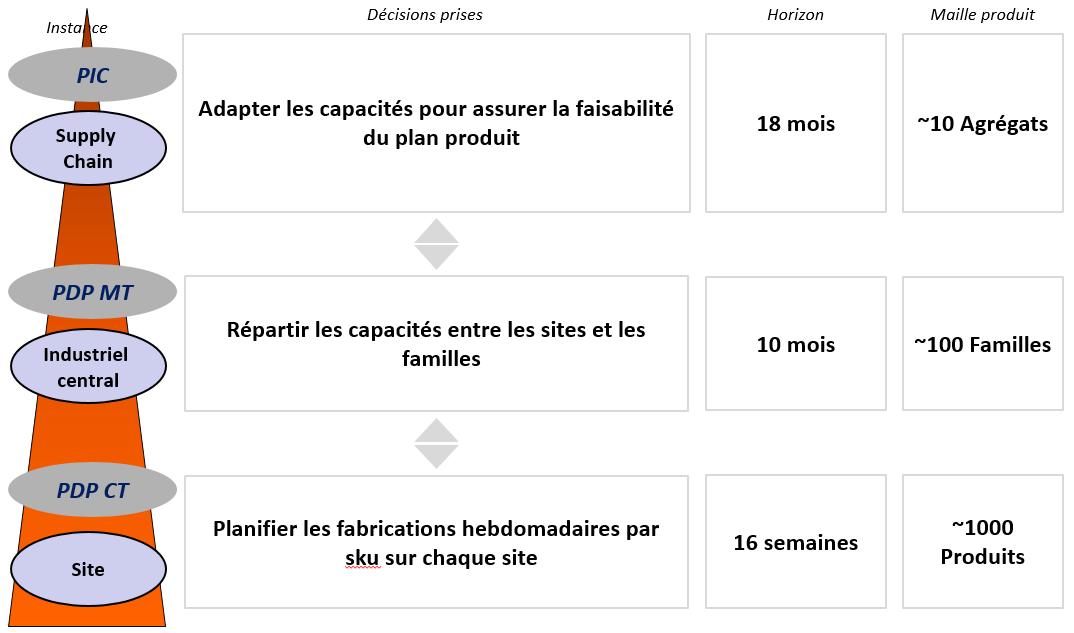
\includegraphics[width=\textwidth]{main/introduction/images/exemple_SC_luxe.png}
  \caption{Exemple d'organisation de la Supply Chain d'un acteur du luxe}
  \label{fig:exemple-SC-luxe}
\end{figure}


\section{Conséquences et problèmes étudiés}


Optimsation multi-objectif : triangle coût / stock / service. (coût = coût hors stock).


2 sujets traités:
\begin{itemize}
  \item le niveau de multi-sourcing (moyen terme).
  \begin{itemize}
    \item Objectif : minimiser les coût de la création du multi-sourcing
    \item Contrainte : taux de service client
    \item Décisions : affectation produits / site
  \end{itemize}
  \item la plannification sous contrainte de flexibilité (court terme) décliné en deux axes :
  \begin{itemize}
    \item Optimization des paramètres des outils de PDP
    \begin{itemize}
      \item Objectif : minimiser le coût du stock
      \item Contrainte : flexibilité industrielle (nombre de changements)
      \item Décisions : Couverture de la production de chaque produits
    \end{itemize}
    \item Création du PDP en intégrant directement la contrainte de flexibilité
    \begin{itemize}
      \item Objectif : minimiser le coût du stock
      \item Contrainte : flexibilité industrielle (nombre de changements)
      \item Décisions : période de production et quantité produite pour chaque produit
    \end{itemize}
  \end{itemize}
\end{itemize}


Parler de la flexibilité du mix produit ! C'est ce qu'on optimise (ie : volume constant.)